%TC:group longtable 0 0

\chapter{Optimising resource allocation in MEC}\label{ch:proposed-solution}
In chapter~\ref{ch:project-problem}, the problem that this project aims to address was outlined along with a short
description of the proposed solution. This chapter builds upon that, giving a formal mathematical model for the problem
in section~\ref{sec:optimisation-problem}. Section~\ref{sec:auctioning-of-tasks} proposes an auction mechanism in order
to pay servers for their resources in order to deal with self-interested users and as server are payed for use of their
services. \\
Using the optimisation problem and auction mechanism from the previous sections, agents for both auction and resource
allocation are proposed, in section~\ref{sec:proposed-agents}, that learns together to maximise a server's profits
over time.

\section{Resource allocation optimisation problem}\label{sec:optimisation-problem}
Using the flexible resource principle, the time taken for a operation to occur, e.g.\ loading of a program, computing
the program and sending of results, etc, is proportional to the amount of resources allocated to complete the operation.
A modified version of a resource allocation optimisation model can be formatted by building upon a similar formulation
in~\cite{FlexibleResourceAllocation}.

A sketch of the whole system is shown in figure~\ref{fig:system_model}.
The system is assumed to contain a set of $I = \{1,2,\ldots,\left|I\right|\}$ servers that are heterogeneous in all
characteristics. Each server has a fixed resource capacity: storage for the code/data needed to run a task
(e.g., measured in GB), computation capacity in terms of CPU cycles per time interval (e.g., measured in GHz),
and communication bandwidth to receive the data and to send back the results of the task after execution
(e.g., measured in Mbit/s). The resources for server $i$ are denoted: $S_i$ for storage capacity, $W_i$ for computation
capacity, and $R_i$ for communication capacity. The system occurs over time that is defined as the set
$T = \{1,2,\ldots,\left|T\right|\}$.

\begin{wrapfigure}{l}{0.5\textwidth}
    \centering
    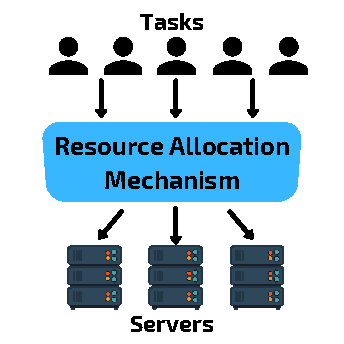
\includegraphics[width=0.5\textwidth]{figures/solution_fig/system_model.pdf}
    \caption{System model}
    \label{fig:system_model}
\end{wrapfigure}

The system is also assumed to contain a set of $J = \{1,2,\ldots,\left| J \right|\}$ heterogeneous tasks that require
services from one of the servers in set $I$. To run any of these tasks on a server requires storing the appropriate
code/data on the same server. This could be, for example, a set of images, videos or Convolutional neural network
layers used in identification tasks.\\
The storage size of task $j$ is denoted as $s_j$ with the rate at which the program is transferred to a server at time
$t$ being $s^{'}_{j,t}$. For a task to be computed successfully, it must fetch and execute instructions
on a CPU. We consider the total number of CPU cycles required for the program to be $w_j$, where the number of
CPU cycles assigned to the task at time $t$ is $w^{'}_{j,t}$. Finally, after the task is run and
the results obtained, the latter needs to be sent back to the user. The size of the results for task $j$ is denoted with
$r_j$, and the rate at which they are sent back to the user is $r^{'}_{j,t}$ on a server at time $t$. \\
The allocation of a task to server is denoted by $x_{i,j}$ for each task $j \in J$ and each server $i \in I$. This is
constrained by equation~\eqref{eq:server_task_allocation} meaning that a task can only be allocated to a single server
at any point in time.

\begin{align}
    \sum_{i \in I} x_{i,j} \leq 1 && \forall{j \in J} \label{eq:server_task_allocation} \\
    x_{i,j} \in \{0, 1\} && \forall{i \in I, j \in J} \label{eq:server_task_binary}
\end{align}

As the task must complete each stage in series, additional variables are required to track the progress of
each task stage. $\hat{s}_{j,t}$ denotes the loading progress of the task, $\hat{w}_{j,t}$ denotes the compute progress
and $\hat{r}_{j,t}$ denotes the sending progress of the task. Each of these variables are updated recursively depending
on the progress in the previous time step plus the resources allocated. Progress is also limited to each of the tasks
total required resources in constraints~\eqref{eq:loading_progress_limit},~\eqref{eq:compute_progress_limit}
and~\eqref{eq:sending_progress_limit}.

\begin{align}
    \hat{s}_{j,t+1} = \hat{s}_{j,t} + s^{'}_{j,t} && \forall{j \in J, t \in T } \label{eq:loading_progress} \\
    \hat{w}_{j,t+1} = \hat{w}_{j,t} + w^{'}_{j,t} && \forall{j \in J, t \in T } \label{eq:compute_progress} \\
    \hat{r}_{j,t+1} = \hat{r}_{j,t} + r^{'}_{j,t} && \forall{j \in J, t \in T } \label{eq:sending_progress} \\
    \hat{s}_{j,t} \leq s_j && \forall{j \in J, t \in T} \label{eq:loading_progress_limit} \\
    \hat{w}_{j,t} \leq w_j && \forall{j \in J, t \in T} \label{eq:compute_progress_limit} \\
    \hat{r}_{j,t} \leq r_j && \forall{j \in J, t \in T} \label{eq:sending_progress_limit}
\end{align}

Every task has an auction time, denoted by $a_j$ and a deadline, denoted by $d_j$. This is the time step when the task
is auctioned and the last time for which the task can be completed successfully. During this time, the time required
to send the data/code to the server, run it on the server, and get back the results to the user which must occur in
order. As a server couldn't start computing a task that was already fully loaded on the machine, for example. A
deadline constraint can simply be constructed such that the sending results progress is finished on the deadline
time step (equation~\eqref{eq:deadline}).

\begin{align}
    \hat{r}_{j, d_j} = r_j && \forall{j \in J} \label{eq:deadline}
\end{align}

As servers have limited capacity, the total resource usage for all tasks running on a server must be capped.
The storage constraint (equation~\eqref{eq:server_storage_capacity}) is unique as the sum of the loading progress for
each task allocated to the server. While the computation capacity (equation~\eqref{eq:server_computation_capacity}) is
the sum of compute resources used by all of the tasks on a server $i$ at time $t$ and the bandwidth capacity
(equation~\eqref{eq:server_bandwidth_capacity}) being less than the sum of resources used to load and send results back
by all allocated tasks.

\begin{align}
    \sum_{j \in J} \hat{s}_{j,t} x_{i,j} \leq S_i, && \forall{i \in I, t \in T} \label{eq:server_storage_capacity} \\
    \sum_{j \in J} w^{'}_{j,t} x_{i,j} \leq W_i, && \forall{i \in I, t \in T} \label{eq:server_computation_capacity} \\
    \sum_{j \in J} (s^{'}_{j,t} + r^{'}_{j,t}) x_{i,j} \leq R_i, && \forall{i \in I, t \in T} \label{eq:server_bandwidth_capacity}
\end{align}

\section{Auctioning of Tasks}\label{sec:auctioning-of-tasks}
%% Auctionsa are common ways of dealing with resources

While the mathematically description of the problem presented in the previous section doesn't consider any auctions
occurring. In real life servers normally wish to be paid for the use of their resources. However due to the modifications
that this project has to make to the optimisation problems, all of the auction mechanisms discussed in
section~\ref{sec:resource-allocation-and-pricing-in-cloud-computing} cannot be used. This is true as the user is not
requesting a fixed amount of resources nor can the available resources be easily computed as this is dynamic, depending
on the different stages of tasks allocated to a server. The modification also affects the algorithms presented
in~\cite{FlexibleResourceAllocation} as they assume that all of the task stages can occur concurrently. This means that
a novel or modified auction mechanism must be used to deal with these changes. Due to the complexities of devising a new
auction mechanism and the large corpus of research on auctions already, outline of the most common auctions is presented
in table~\ref{tab:auctions_descriptions} with their respective properties in table~\ref{tab:auction_properties}.

\begin{longtable}{|p{3.5cm}|p{11cm}|} \hline
    \textbf{Auction type} & \textbf{Description} \\ \hline
    English auction & A traditional auction where all participant can bid on a single item with the price slowly
        ascending till only a single participant is left who pays the final bid price. Due to the number of rounds,
        this requires a large amount of communication. \\ \hline

    Dutch auction & The reverse of the English auction, where the starting price is higher than anyone is willing to
        pay with the price slowly dropping till the first participant "jumps in". This can result in sub-optimal pricing
        if the starting price is not highest enough or a large number of rounds is required till anyone bids. Plus due
        the auctions occurring over the internet, latency can have a large effect on the winner. \\ \hline

    Japanese auction & Similar to the English auction except that the auction occurs over a set period of time with the
        bid increasing over time and last highest bid being the winner. This means that it has the same disadvantages
        as the English auction except that there is no guarantee that the price will converge to the maximum. Plus
        additional factors like latency can have a large effect on the winner and resulting price. But due to the time
        limit, it has a known amount of time till it finishes unlike the English or Dutch auctions. \\ \hline

    Blind auction & Also known as a First-price sealed-bid auction, all participants submit a single secret bid for an
        item with the highest bid winning. As a result there is no dominant strategy (not incentive compatible) as an
        agent would wish to bid only a small amount more than the next highest price in order overpay for the item.
        But due to there being only a single round of biding, latency doesn't affect an agent and allows many
        more auctions could occur within the same time compared to the English, Dutch or Japanese auctions. \\ \hline

    Vickrey auction~\citep{vickrey} & Also known as a second-price sealed bid auction, participants each submit
        a single secret bid for an item with the highest bid winning like the blind auction. However the winner only
        pays the price of the second highest bid. Because of this, it is a dominant strategy (incentive compatible)
        for an agent to bid its true value as even if the bid is much higher than all other participants its doesn't
        matter as they pay the minimum required for them to win. \\ \hline
    \caption{Descriptions of feasible auctions for the project: English, Dutch, Japanese, Blind and Vickrey auction}
    \label{tab:auctions_descriptions}
\end{longtable}

\begin{table}[h]
    \centering
    \begin{tabular}{|l|c|c|c|} \hline
        \textbf{Auction}  & \textbf{Incentive compatible} & \textbf{Number of rounds} & \textbf{Fixed time length} \\ \hline
        English           & False                         & Multiple                  & False            \\ \hline
        Japanese          & False                         & Multiple                  & True             \\ \hline
        Dutch             & False                         & Multiple                  & False            \\ \hline
        Blind             & False                         & Single                    & True             \\ \hline
        Vickrey           & True                          & Single                    & True             \\ \hline
    \end{tabular}
    \caption{Properties of the auctions described in Table~\ref{tab:auctions_descriptions}}
    \label{tab:auction_properties}
\end{table}

The auction properties that this project considers most important is the auction time length and incentive compatibility.
This is as, online auction wish to be fast that is incompatible with the English, Dutch and Japanese auctions and
incentive compatible means that an optimal strategy actually exists to player to play towards. Because of these two
properties, the Vickrey auction~\citep{vickrey} has been chosen. An additional advantage of using the Vickrey auction,
with reinforcement learning agent, is that as it is incentive compatible, agents dont need to learn how to outbid
another agent. They only needs learn to effectively evaluate each task instead of through demand meaning that allowing
agents to possibly learn through self-play.

However a modification must be made due to servers generate the prices for tasks rather than task suggesting a price to servers.
Because of this, the auction is reversed, such that the bid with the minimum price wins the task instead of the maximum
price. The auction therefore works by allowing all servers to submit their bids for a task with the winner
being the server with the lowest price, with the task actually paying second lowest price.

\section{Auction and resource allocation agents}\label{sec:proposed-agents}
Using the optimisation formulation and auction mechanism from the previous two sections, the problem can be modelled as
Markov Decision Process~\citep{Bel} which allows the environment to be model as figure~\ref{fig:mdp_system_model}.
This separates out the auction and resource allocation part of the problem with
separate agents into almost similar environments to act during their respective part of the problem.
Subsection~\ref{subsec:proposed-auction-agents} and~\ref{subsec:proposed-resource-allocation-agents} proposes agents
for the auction environment and resource allocation environment respectively.

\begin{figure}
    \centering
    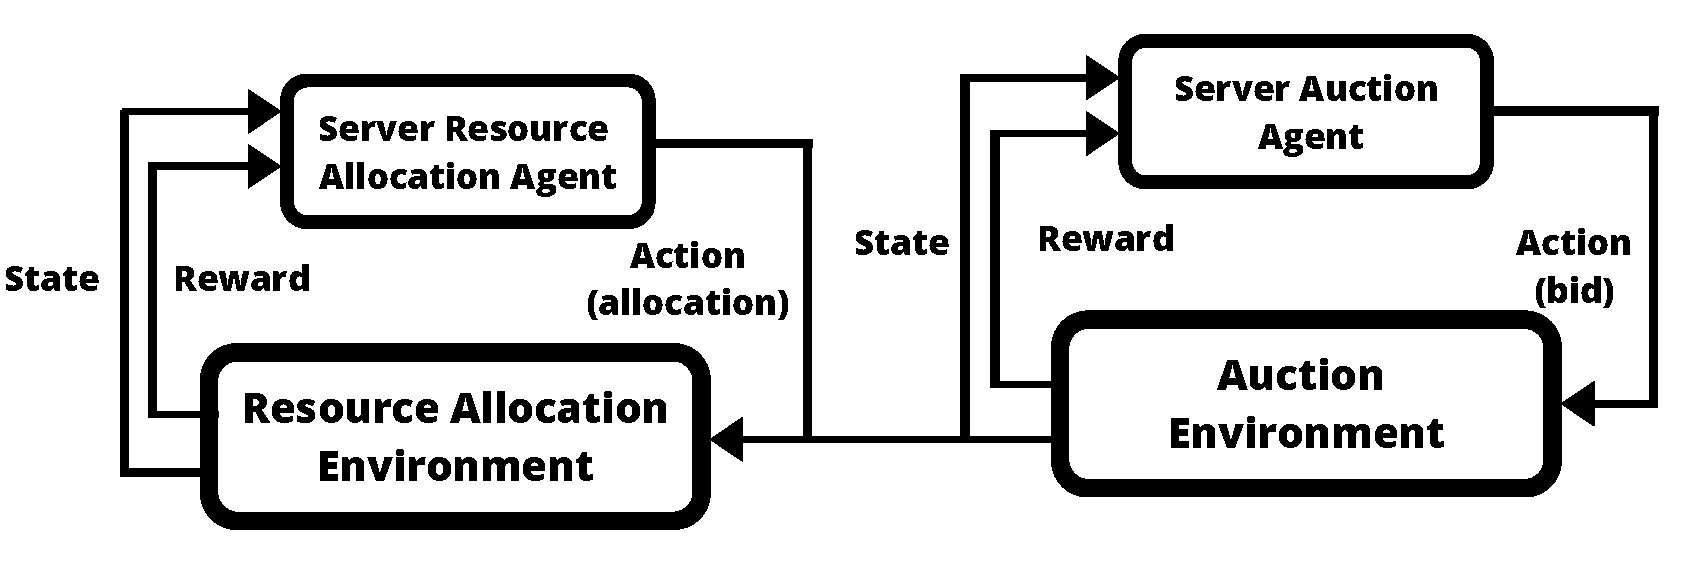
\includegraphics[width=14cm]{figures/solution_fig/flexible_resource_allocation_env.pdf}
    \caption{Markov Decision process system model}
    \label{fig:mdp_system_model}
\end{figure}

The environment is believed to possibly be of interest for multi-agent reinforcement learning researchers as the aim
of the environment is cooperative (to maximise the social welfare) but knowing that servers can act self-interestedly
during the auctions in order to maximise their private profits. But the resource allocation agent must work
cooperatively in allocating of resources for each task as the server wishes to complete as many tasks as they can.
This author believes that this type of environment is unique within reinforcement learning.

\subsection{Proposed auction agents}\label{subsec:proposed-auction-agents}
Traditionally pricing mechanisms~\citep{al2013cloud} rely on mixture of metrics: resource availability, resource demand,
quality of service, task resource requirements, task resource allocation quantity, etc to determine a price. However
these values are difficult to approximate during the auction with this program case. So due to the complexity of
deriving this function, reinforcement learning will be used with the aim to learn an optimal policy to maximise the
profits of the server over time. Simple heuristics will also be implemented in order compare the effectiveness of the
reinforcement learning to untrained heuristics.

\begin{longtable}{|p{3.5cm}|p{10cm}|} \hline
    \textbf{Neural Network} & \textbf{Description} \\ \hline
    Artificial neural networks~\citep{ANN} & Originally developed as a theoretically approximation for the brain, it
        was found that for networks with at least one hidden layer, neural networks could approximate any
        function~\citep{csaji2001approximation}. This made neural networks extremely helpful for cases where it would
        normally be too difficult for a human to specify the exact function as they can be trained through gradient
        descent and supervised learning to find a close approximation to the true function. \\ \hline

    Recurrent neural network~\citep{RNN} & A major weakness of artificial neural networks is that it must use a fixed
        number of inputs and outputs making it unusable with text, sound or video where previous data is important
        for understanding the inputs. Recurrent neural network's extend neural networks to allow for connections to
        previous neurons to "pass on" information. However recurrent neural networks struggle from vanishing or
        exploding gradient during training. \\ \hline

    Long/Short Term Memory~\citep{LSTM} & While recurrent neural network's can "remember" previous inputs to the
        network, it also struggles from the vanishing or exploding gradient problem where gradient tends to zero or
        infinity making it unusable. LSTM aim to prevent this by using forget gates that determines how much
        information the next state will get, allowing for more complexity information to be learnt compared to
        recurrent neural networks. \\ \hline

    Gated Recurrent unit~\citep{GRU} & Gated recurrent unit are very similar to long/short term memory, except for the
        use of a different wiring mechanisms and the one less gate, an update date instead of two forgot gates.
        These changes mean that gated recurrent units run faster and are easier to code than long/short term memory,
        however are not as expressive meaning that less complex functions can be encoded. \\ \hline

    Neural Turing Machine~\citep{NTM} & Inspired by computers, neural turing machines build on long/short term memory
        by using an external memory module instead of memory being inbuilt to the network. This allows for external
        observers to understand what is going on much better than other networks due to their black-box nature. \\ \hline

    Differentiable neural computer~\citep{DNC} & An expansion to the neural turing machine that allows the memory
        module to scalable in size allowing for additional memory to be added if needed. \\ \hline
    \caption{Neural network layer descriptions}
    \label{tab:neural_network_layers}
\end{longtable}

As the action space of the agent is continuous, a deep deterministic policy gradient~\citep{ddpg} agent
will be implemented. The action shape can also be discretized allow deep Q learning agents~\cite{atari} to be trained
as well. In order to compare alternative learning methods and the affect of discretizing the action space on results,
agents will use neural networks as it is known to be able to approximate any
function~\citep{csaji2001approximation}. Because of this, a long/short term memory~\citep{LSTM} layer will be used as
it allows for multiple inputs, and outputs are single vector that will have several additional layers to allow
additional complexity. The network will end at a single ReLU neuron for DDPG or multiple logit activation neurons for
DQN agents as shown in Figure~\ref{fig:task_pricing_network_architecture}.

\begin{figure}
    \centering
    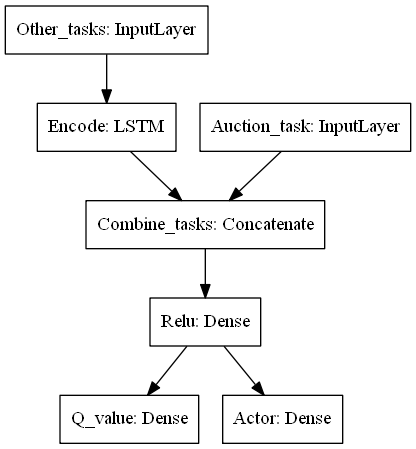
\includegraphics[width=0.5\textwidth]{figures/solution_fig/task_pricing_network_architecture.png}
    \caption{Task pricing network architecture}
    \label{fig:task_pricing_network_architecture}
\end{figure}

\subsection{Proposed resource allocation agents}\label{subsec:proposed-resource-allocation-agents}
When a new task is allocated to the server or a task completes a stage, server resource need to be redistributed
to the task. As the problem of how to allocation resources isn't as complex as the agent pricing in
section~\ref{subsec:proposed-auction-agents}, both simple heuristics and reinforcement learning agents will be
implemented in order to compare effectiveness.

However a similar problem exists as with the proposed auction agents (in subsection~\ref{subsec:proposed-auction-agents}).
Due to knowing how to allocate resources to a single task requires being aware of the resource requirements of other
tasks and how they are being weighted on the server. Therefore a similar network is proposed to allow for the other tasks
to be passed into the network at the same time it is weighting a task. This is shown in
figure~\ref{fig:resource_weighting_network_architecture}

A weighting heuristic is proposed for the network output as well, such that the network doesn't output the raw
resources allocated for a task but rather a weighted value for the resources needing to allocated for the task.
This has the advantage of being a simpler function to approximate for agents but with a similar expressiveness as an
exact resource usage function. This also avoids the problem of the network either over allocating the resources to tasks
or severely under allocating resources.

\begin{figure}
    \centering
    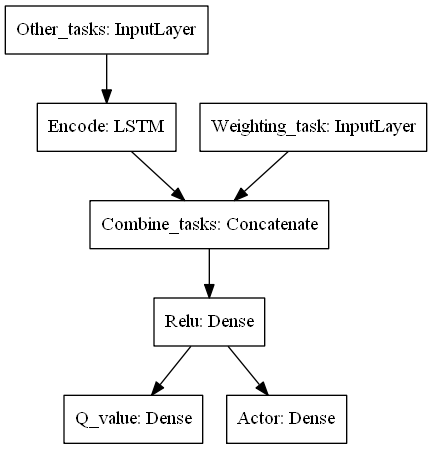
\includegraphics[width=0.5\textwidth]{figures/solution_fig/resource_weighting_network_architecture.png}
    \caption{Resource weighting network architecture}
    \label{fig:resource_weighting_network_architecture}
\end{figure}


